\documentclass[12pt]{TD-CJS}
\renewcommand{\baselinestretch}{2}
% started December 2019...after editor's comments on 2nd revision ; minor edits
 
\usepackage{latexsym}
\usepackage{amsmath}
\usepackage{amsfonts}
\usepackage{amssymb}
\usepackage{psfrag}
\usepackage{graphicx}
\usepackage{enumitem}
\usepackage{algorithm}% http://ctan.org/pkg/algorithms
\usepackage{algpseudocode}% http://ctan.org/pkg/algorithmicx
\usepackage{multirow}
\usepackage{dsfont}




\newcommand{\prox}{ \mathop{\mathrm{prox}} }
\newcommand{\R}{\mathcal{R}}
\newcommand{\defeq}{\mathrel{\mathop:}=}
\newcommand{\eqdist}{\stackrel{D}{=}}

\DeclareMathOperator*{\argmax}{arg\,max} 
\DeclareMathOperator*{\argmin}{arg\,min} 

\newcommand{\pushcode}[1][1]{\hskip\dimexpr#1\algorithmicindent\relax}
\begin{document}
%\rhauthor{Michael A. Newton,  Nicholas G. Polson and Jianeng Xu}
\rhauthor{Blinded-A, Blinded-B, and Blinded-C}
\copyrightline{Statistical Society of Canada}
\Frenchcopyrightline{Soci\'et\'e statistique du Canada}


\title[Weighted Bayesian Bootstrap]{Weighted Bayesian Bootstrap for Scalable Posterior Distributions 
 \footnotetext{We would like to thank the associate editor and referees for their detailed, helpful comments.}}
%\author{Michael A. Newton\authorref{1}}
%author{Nicholas G. Polson\authorref{2}}
%\author{Jianeng Xu\authorref{3}}
%\affiliation[1]{Departments of Statistics and of Biostatistics and Medical Informatics, University of Wisconsin-Madison}
%\affiliation[2]{Booth School of Business, University of Chicago}
%\affiliation[3]{Booth School of Business, University of Chicago}
\author{Blinded-A}
\author{Blinded-B}
\author{Blinded-C}


\startabstract{
\keywords{
\KWDtitle{Key words and phrases}
Bayesian\sep Bootstrap\sep Markov chain Monte Carlo\sep Weighted Bootstrap\sep Approximate Bayesian Computation\sep Trend Filtering\sep Deep Learning\sep Regularization.
% MSC 2010 subject classification codes
\KWDtitle{MSC 2010}Primary 62F40\sep secondary 6262F15}
\begin{abstract}
\abstractsection{}
\abstractsection{Abstract}
We introduce and develop a Weighted Bayesian Bootstrap (WBB) for  Machine Learning and Statistics. WBB provides uncertainty quantification by sampling from a high dimensional posterior distribution. WBB is computationally fast and scalable using only off-the-shelf optimization software.  First-order asymptotic analysis provides a theoretical justification
under suitable regularity conditions on the statistical model.
We illustrate the proposed
methodology in regularized regression, trend filtering and deep learning and conclude with directions for future research.

\end{abstract}}
\makechaptertitle


\newpage

\section{Introduction}
Weighted Bayesian Bootstrap (WBB) is a simulation-based algorithm for assessing uncertainty in Machine Learning and Statistics. Uncertainty quantification (UQ) is an active area of research, particularly in high-dimensional inference problems (Wang and Swiler, 2018). 
Whilst there are computationally fast and scalable algorithms for training models in a wide variety of contexts, uncertainty assessments are still required, as are methods to compute these assessments.  Bayesian analysis offers a general solution, but developing computationally fast scalable algorithms for sampling a posterior distribution is a notoriously hard problem. WBB makes a contribution to this literature by showing how off-the-shelf optimization algorithms, such as convex optimization or stochastic gradient descent (SGD), can be adapted to provide uncertainty assessments. Our goal here is to marry Bayesian uncertainty techniques with state-of-the-art optimization methods 
and software systems.
 
For relatively simple statistical models, the weighted likelihood bootstrap (WLB) method provides
approximate posterior sampling through repeated optimization of a randomly weighted likelihood function (Newton and Raftery, 1994).
The proposed WBB extends the WLB to a broad class of  contemporary statistical models by leveraging advances in optimization methodology.
Essentially, the WLB used optimization of certain 
randomized objective functions to enable approximate marginalization ({\em i.e.}, integration) 
required in Bayesian analysis.  The same idea -- optimize a randomized objective function to 
achieve  posterior sampling -- is at the heart of the proposed WBB method, though some changes to the WLB procedure are required to 
carry out this program for the models considered.
Theoretical support for the WLB approximation is based on  connections between posterior variation and curvature of 
the log-likelihood revealed through repeated optimization of randomly weighted likelihoods. 
 By contrast, the proposed WBB calculates a series of
randomized  posterior modes rather than randomized likelihood maximizers. A key rationale for this proposal is  that 
high dimensional posterior modes are now readily computable, thanks to systems such as \verb+TensorFlow+ (Abadi {\em et al.}, 2015) and 
\verb+Keras+ (Chollet {\em et al.}, 2015)
that deploy stochastic gradient descent (SGD) and convex optimization methods for large-scale
problems, such as on neural network architectures used in deep learning (LeCun {\em et al.}, 2015).
By linking random weighting with modern-day optimization, we expose a simple scheme
for approximate uncertainty quantification in a wide class of statistical models.

Quantifying uncertainty is typically unavailable in a purely regularization optimization method. 
We contend that UQ is available directly by repeated optimization of randomized objective functions, using the same
computational tools that produce the primary estimate,  rather than through Markov
chain Monte Carlo, variational methods,  approximate Bayesian computation, or other techniques. See Green {\em et al.} (2015) for a good summary of Bayesian computation history. Thus, uncertainty assessments are provided at little extra effort over the original
training computations.  A further benefit is that with extra computational cost, it is straightforward to add a regularization path 
across hyper-parameters (e.g., simply repeat WBB on different $\lambda$), which is usually difficult to compute in traditional Bayesian
sensitivity analysis.  We use predictive cross-validation techniques in this regard.

The rest of the paper is outlined as follows. Section 2 develops our weighted Bayesian Bootstrap (WBB) algorithm. Section 3 provides applications to high dimensional sparse regression, trend filtering and deep learning. WBB can also be applied to Bayesian tree models (Taddy {\em et al.}, 2015).  Section 4 indicates several directions for future research, 
including bootstrap filters in state-space models (Gordon {\em et al.},  1993)  and connections to the resampling-sampling
perspective in sequential Bayesian inference (Lopes {\em et al.}, 2012).

\section{Weighted Bayesian Bootstrap}
\subsection{Set up}
We work with a broad class of statistical models for data structures involving outcomes and covariates.
Examples considered in Section~3  include  regression, trend-filtering, and deep learning.
Let  $y=(y_1, y_2, \cdots, y_n)$ be an $n$-vector of outcomes and let $\theta = (\theta_1, \theta_2, ..., \theta_p)$ be a $p$-dimensional parameter of interest. 
Covariate data may be organized in an 
$n \times p$ matrix $A$ whose rows are the design points (or ``features'') $a_i^T$
where we index  observations by $i$ and parameters by $j$.  
A large number of estimation/training  problems can be expressed in the form
\begin{equation}
\label{eqn:canonicalform}
\begin{aligned}
& \underset{\theta \in \R^d}{\text{minimize}}
& &  \mathcal{L}(\theta) \defeq l(y| \theta) + \lambda\phi(\theta) \, ,
\end{aligned}
\end{equation}
where $l(y| \theta) = \sum_{i=1}^n l_i( y_i | \theta )$ is a measure of fit (or ``empirical risk function'') depending on $\theta$ and $y$ and implicitly on $A$.
The penalty function, or regularization term, $\lambda\phi(\theta) $,   
may encode soft or hard constraints, and is controlled by 
a hyper-parameter, $\lambda>0$, whose values index an entire path of solutions. 
The penalty function $\phi(\theta)$ effects a favorable bias-variance 
estimation tradeoff and provides extensive modeling flexibility (Wellner and Zhang, 2012).   
To accommodate contemporary applications we  allow $\phi(\theta)$ to have points in its domain where it fails to be differentiable (e.g., $L^1$ norm).  
If we treat data, $y$, as arising from a probabilistic 
model parameterized by $\theta$, then the likelihood function $p(y|\theta)$ yields 
the model-associated measure of fit $l(y| \theta) = -\log p(y|\theta)$.
The maximimum likelihood estimator (MLE) is  $ \hat{\theta} \defeq {\rm arg max}_\theta\; p(y |\theta) $, though
of course this usually differs from the solution to~(\ref{eqn:canonicalform}): $\theta^* \defeq \argmin \left\{ l(y|\theta) + \lambda \phi(\theta)
 \right\}]$.  We recall a key duality between regularization and Bayesian analysis.

% and, relative some prior $p(\theta)$,
%\begin{enumerate}[label=(\roman*)]
%\item let $\theta^*_n \defeq {\rm arg max}_\theta \; p( \theta|y) $ be the posterior mode,
%\item let $ \bar{\theta}_n \defeq E(\theta | y) $ be the posterior mean.
%\end{enumerate}
%Next, we recall a key duality between regularization and Bayesian analysis.

\subsection{Bayesian Regularization Duality}

From the Bayesian perspective, the measure of fit, $l(y|\theta) = - \log p(y| \theta)$, and the penalty function, $\lambda\phi(\theta)$, correspond to the negative logarithms of the likelihood and prior distribution in the model
\begin{equation}
\label{eqn:bayes}
\begin{aligned}
 p(y | \theta) \propto \exp & \{-  l(y|\theta)\} \; , \quad p(\theta) \propto \exp\{ - \lambda\phi(\theta) \} \\
p( \theta | y ) &  \propto \exp\{- ( l(y|\theta) + \lambda\phi(\theta) ) \}.
\end{aligned}
\end{equation}
This posterior $p(\theta|y)$  is often a proper distribution over $\R^d$, even if the prior $p(\theta)$ is not proper. 
The well-known equivalence between regularization and Bayesian methods is seen,
for example, in regression with a Gaussian regession model
subject to a penalty such as an $L^2$-norm (ridge) Gaussian prior or $ L^1$-norm (LASSO) 
double exponential prior.  By this duality, the posterior mode, or maximum a posteriori (MAP) estimate, is $\theta^*$,  
a solution to~(\ref{eqn:canonicalform}).
%\begin{eqnarray}
%\theta^* & =& \underset{\theta \in \Theta}{\argmin}\,  \{ l(y|\theta) + \lambda\phi(\theta) \}.  \label{posteriormode}
%\end{eqnarray}
See Gribonval and Machart (2013) for a nuanced view of the connection between~(\ref{eqn:canonicalform}) and~(\ref{eqn:bayes}) in
Gaussian regression models. 

\subsection{Optimization}

Advances in optimization methodology provide efficient algorithms
to compute $\theta^* = \argmin \mathcal{L}(\theta)$  for a wide range of  loss and penalty functions. 
Theory is well developed in the case of convex objective functions (e.g., Bertsekas {\em et al.}, 2003; Boyd and Vandenberghe, 2004). For example
if loss $l$ is convex and differentiable in $\theta$ and penalty $\phi$ is convex, then 
a necessary and sufficient condition for $\theta^*$ to minimize $ l(y|\theta) + \lambda\phi(\theta)$  is 
\begin{equation}
\label{eqn:subdiffproxgrad}
0 \in \partial \left\{ l(y|\theta^*) + \lambda\phi(\theta^*)\right\} = \nabla l(y|\theta^*) + \lambda\partial \phi(\theta^*) 
\end{equation}
where $\partial$ is the subdifferential operator (the set of subgradients of the objective), in this case
the sum of a point and a set.   Though not a formula for $\theta^*$, such as given by the normal equations in linear regression, 
(\ref{eqn:subdiffproxgrad}) usefully guides algorithms that aim to solve $\theta^*$.   
For example, under separability conditions on the penalty function, coordinate descent algorithms effectively solve for $\theta^*$;
see Wright (2015), or  Hastie {\em et al.} (2015, chap. 5) for a statistical perspective.
The optimization literature also characterizes $\theta^*$ as the fixed point of a proximal operator
$\prox_{\gamma \mathcal{L}}(\theta) = \argmin_z \{ \mathcal{L}(z) - \frac{1}{2\gamma} || z - \theta||_2^2  \}$, 
which opens the door to powerful MM algorithms and related schemes; 
 see Lange (2016, chap. 5), Polson and Scott (2015), and Polson {\em et al.} (2015).  
Beyond convexity, the guarantees are weaker (e.g., local
not global minima) and the algorithms are many (e.g., Nocedal and Wright, 2006).  Gradient descent
or stochastic gradient descent (SGD) are effective in many cases, owing to parameter 
dimensionality and structure of the gradients.  The appendix develops SGD for one example.

Advances in applied optimization provide effective software tools for data analysis. For example, the R package
\verb+glmnet+ deploys coordinate descent for loss functions arising from generalized linear models and LASSO or 
elastic net penalties (Friedman {\em et al.}, 2010). To solve the generalized LASSO problem, the R package 
\verb+genlasso+  deploys a dual path algorithm (Arnold and Tibshirani, 2014).  A variety of general 
purpose optimization tools for statistics are compiled at the optimization view at CRAN 
(\verb+https://cran.r-project.org/web/views/Optimization.html+). For machine learning, the \verb+TensorFlow+ system has greatly simplified 
gradient descent, SGD, and related algorithms for many applications (Abadi {\em et al.}, 2015).  




\subsection{WBB Algorithm}
\noindent We now define the weighted Bayesian Bootstrap (WBB).  Recalling the original objective function~(\ref{eqn:canonicalform}),
we form the randomized objective
\begin{eqnarray}
\label{eqn:rand}
\mathcal{L}_{\bf w}( \theta ) = \left\{ \sum_{i=1}^n w_i l_i( y_i | \theta ) \right\} + \lambda w_0 \phi(\theta)
\end{eqnarray}
%$$
%{\bf w} = (w_1, ..., w_n, w_p),\,
%p_{\bf w}(\theta | y) \propto \prod_{i=1}^n p(y_i|\theta)^{w_i} p(\theta)^{w_p}
%$$
where entries of  ${\bf w}=(w_0, w_1, \cdots, w_n)$ are independent and identically distributed (i.i.d.) 
standard exponentially distributed random weights, generated by the analyst and independently from the data $y$. 
Equivalently, 
$w_i = \log(1/u_i)$ where $u_i$'s are i.i.d. Uniform$(0,1)$. When $p$ is relatively large
 and $\phi(\theta)$ is separable as $\phi(\theta) = \sum_{j=1}^p \phi_j(\theta_j)$, we 
recommend an extension in which $w_0=(w_{0,1}, w_{0,2}, \cdots, w_{0,p})$ 
allows separate i.i.d. random  weights on the prior regularization terms $\phi_j(\theta_j)$, namely $\lambda \sum_{j=1}^p w_{0,j} \phi_j(\theta_j)$, to help with sparsity and to reduce the effect of occasionally large scalar weight.
In either case, associated with any vector ${\bf w}$ is the solution,
$\theta^*_{\bf w} = \argmin \mathcal{L}_{\bf w}(\theta).$
Our basic conjecture is that the conditional distribution of $\theta^*_{\bf w}$ -- the distribution
induced by ${\bf w}$ with the data fixed --  approximates the Bayesian posterior~(\ref{eqn:bayes}). For any measurable set $\mathcal{B}$ in the parameter space,
\begin{eqnarray}
\label{eqn:conjecture}
{\rm Pr}\left( \theta^*_{\bf w} \in \mathcal{B} | y \right) \approx \int_\mathcal{B} p(\theta|y) \, d\theta.
\end{eqnarray}
Section 2.5 provides an asymptotic argument in support of~(\ref{eqn:conjecture}), and we investigate
the approximation numerically in a few examples in Section 3.   Assuming this conjecture is true, we have immediately 
a straightforward, optimization-based algorithm for approximate posterior sampling:

% We note that rescaling in~(\ref{eqn:rand}) has no effect on 
%solutions~(\ref{eqn:wbb}), and so it is equivalent in the construction 
% to use normalized weights $\tilde {\bf w}$ that sum to unity. Such $\tilde {\bf w}$ are uniformly distributed over
%the $(n+1)$-dimensional unit simplex, and thus have a specific Dirichlet distribution.


%We have used the fact that for i.i.d. observations, the likelihood can be factorized as $p(y|\theta) = \prod_{i=1}^n p(y_i|\theta)$. This is not crucial for our analysis but is a common assumption. Let $\theta^*_{{\bf w},n}$ denote the mode of this regularized distribution. Again, there is an equivalence 

%$$
%\theta^*_{{\bf w},n} := \underset{\theta}{\argmax} \; p_{\bf w}(\theta | y) \equiv \underset{\theta}{\argmin} \sum_{i=1}^n w_i l_i(y_i|\theta) + \lambda w_{p} \phi(\theta)
%$$
%where $l_i(y_i|\theta) = -\log p(y_i|\theta)$ and $ \lambda\phi(\theta) = -\log p(\theta)$. Note that we have a weighted likelihood and a new regularization parameter, $\lambda w_p$.



\begin{algorithm} [H]
        \caption{Weighted Bayesian Bootstrap}
        \label{alg:ALG1}
        \textbf{Input:}  \begin{list}{}
                         \item data: ${\mathcal D}=(y,A)$ 
                         \item model structure: ${\mathcal M}=\left( \{l_i\} ,\lambda,\phi\right)$ 
                         \item number of draws: $T$ 
	                \end{list}
        \textbf{Output:} $T$ parameter samples $\{ \theta^{*,t} \}$
        \begin{algorithmic}
            \State  Function ${\bf WBB}({\mathcal D},{\mathcal M},T)$:

            \ForAll  {$t=1$ to $T$}
		\State Realize: $(u_1, \cdots, u_n) \sim_{i.i.d.}\, $Uniform$(0,1)$ 
		\State Construct: $w_i \gets \log(1/u_i), \forall i. $
		\State Independently construct $w_0$ as either a univariate Exponential
  (common weight case) or as a vector of i.i.d. Exponentials (separate weights case)
		\State Set ${\bf w}=(w_0, w_1, \cdots, w_n)$ 
		\State Compute: $\theta^{*,t} \gets \argmin {\mathcal L}_{\bf w}(\theta)$

            \EndFor 

        \end{algorithmic}
    \end{algorithm}


%\noindent  The crux of our procedure is to create a sample of the weighted posterior modes $\{ \theta_{{\bf w},n}^*\}$ (computationally cheap as each sub-problem can be solved via optimization). Our main result is the following:\\
%\textbf{Algorithm: Weighted Bayesian Bootstrap (WBB)}
%\begin{enumerate}
%\item Iterate: sample ${\bf{w}} = \{w_1, w_2, ..., w_n, w_p\}$ via exponentials. $w_p, w_i\sim Exp(1)$. 
%\item For each ${\bf{w}}$, solve $\theta^*_{{\bf w},n} = \underset{\theta}{\argmin} \sum_{i=1}^n w_i l_i(\theta) +  \lambda w_p \phi(\theta)$. 
%\end{enumerate}

When optimization on the original problem~(\ref{eqn:canonicalform}) is fast and scalable, so too is the WBB. Weights ${\bf w}$ and the corresponding  $\theta^*_{\bf w}$ are independent across $t$, making it possible to speed up the algorithm via parallel computing.
To choose the amount of regularization $\lambda$ which is assumed to be fixed for all sets of ${\bf w}$, we can use the marginal likelihood $m_\lambda (y)$, estimated by bridge sampling (Gelman and Meng, 1998) or simply using predictive cross-validation.
Next we consider the approximation~(\ref{eqn:conjecture}) from an asymptotic perspective.

% The WBB algorithm is fast and scalable to compute a regularized estimator. For a large number of popular priors, the minimizing solution $\theta^*_{{\bf w},n}$ in the second step can be directly obtained via regularization packages such as {\tt glmnet} by Trevor Hastie and {\tt genlasso} by Taylor Arnold, see  \cite{friedman2010regularization} and \cite{arnold2014genlasso}. When the likelihood function or the prior is specially designed, Stochastic Gradient Descent (SGD) is powerful and fast enough to solve the minimization problem. It can be easily implemented in TensorFlow once the objective function is specified. 


\subsection{WBB Properties}

Conditions under which the target posterior distribution~(\ref{eqn:bayes}) is approximately Gaussian are well established (Kleijn and van der Vaart, 2012).  For example, when data form a random sample from fixed distribution $p(y_i|\theta_0)$
that resides in a sufficiently regular model, and when the prior is smooth and positive around $\theta_0 \in \R^p$,  we have 
\begin{eqnarray}
\label{eq:postG}
\left. \theta \right| y  \sim_{\rm approx} N_p \left( \theta_n^*, J_n^{-1}(\theta^*_n)\right),
\end{eqnarray}
where, including sample size $n$ as an explicit subscript, we have posterior mode $\theta_n^* = \argmin {\mathcal L}_n( \theta)$, and
where $J_n(\theta^*_n)=nj(\theta_n^*)$ is the Fisher information matrix evaluated at $\theta_n^*$.  
Here $j(\theta)$ is the information per sample, and $y=(y_1, \cdots, y_n)$ denotes data. Johnstone (2010) studies Bernstein-von Mises theorem in high dimensional settings where $p$ grows with $n$ and the situation is very different. 
Centering on the posterior mode, rather than the MLE, improves accuracy in many cases (Bertail and Lo, 1991).   


As to the WBB distribution, consider a one-term Taylor expansion of $\nabla {\mathcal L}_{{\bf w},n} (\theta)$ about the posterior
mode $\theta^*_n$, which is allowable for sufficiently smooth loss and penalty terms:
\begin{eqnarray}
\label{eq:wbbTaylor}
\nabla {\mathcal L}_{{\bf w}, n} (\theta) = \nabla {\mathcal L}_{ {\bf w}, n}( \theta^*_n ) + 
 \nabla^2 {\mathcal L}_{ {\bf w}, n }(\theta_n^*)  (\theta - \theta^*_n )  + R_n
\end{eqnarray}
where $R_n$ is an error term and $\nabla$ and $\nabla^2$ record the gradient vector and matrix of second partial
derivatives, respectively, of the weighted objective function.  Evaluating this expansion at $\theta^*_{ {\bf w}, n } = \argmin {\mathcal L}_{{\bf w},n}(\theta)$ zeros
out the left hand side of~(\ref{eq:wbbTaylor}) and leads to:
\begin{eqnarray}
\label{eq:asymp}
\sqrt{n} \left( \theta_{{\bf w},n }^* - \theta_{n}^*  \right) = - \left( \frac{1}{n} \nabla^2 {\mathcal L}_{{\bf w},n} ( \theta^*_n )  \right)^{-1} \left(  \frac{1}{\sqrt{n}}
     \nabla {\mathcal L}_{{\bf w},n} ( \theta_n^* )  \right)  + \tilde R_n 
\end{eqnarray}
where $\tilde R_n$ is another error term.  Following Newton and Raftery (1994), we recognize that the ${\bf w}$-induced variation in~(\ref{eq:asymp}), conditional upon 
the data, causes the matrix factor to be approximately the inverse information 
$[J_n(\theta^*_n)]^{-1}$, the score-like second factor to be approximately mean-zero 
Gaussian with covariance equal to $J_n(\theta^*_n)$, and the error $\tilde R_n$ to be
negligible.   Thus, compared to the target posterior variation~(\ref{eq:postG}), we 
have WBB variation:
\begin{eqnarray*}
\left. \theta^*_{{\bf w},n} \right| y  \sim_{\rm approx} N_p \left( \theta_n^*, J_n^{-1}(\theta^*_n)\right).
\end{eqnarray*}
In a relatively narrow asymptotic sense, therefore, the WBB procedure is approximating the
target posterior distribution, as both are approximately Gaussian with the same mean
and covariance.   Details of the asymptotic analysis follow the WLB case presented in 
Newton and Raftery (1994), 
and differ only slightly in our use of the posterior mode $\theta^*_n$ in place
of the maximum likelihood estimator $\hat \theta_n$, and also in our incorporation of weight
$w_0$ on the penalty term of the objective function.   At this level of first-order 
 asymptotic analysis, neither of these features affects the limiting conditional
Gaussian distribution of $\theta^*_{{\bf w},n}$.



%{\it Nick,   you wrote *$J_n = nj$ as `observed information`, but if it's the curvature of the observed log likelihood then I guess it's not $n j$.  Do you mean Fisher information?**}



%The following proposition, which follows from the Theorem 2 in Newton and Raftery (1994), summaries the properties of WBB.
%
%\begin{proposition}{Proposition}{}
%The weighted Bayesian Bootstrap draws are approximate posterior samples
%$$
%\left\{\theta^{*(k)}_{{\bf w},n} \right\}_{k=1}^K \sim p(\theta | y).
%$$
%\end{proposition}
%%
%Now we consider `large $n$' properties. The variation in the posterior density $p(\theta|y) \propto e^{-n l_n(\theta)}p(\theta)$ for sufficiently large $n$ will be dominated by the likelihood term. Expanding $l_n(\theta)$ around its maximum, $\hat\theta$, and defining $J_n(\hat\theta) = nj(\hat\theta)$ as the observed information matrix gives the traditional normal approximation for the posterior distribution
%$$
%\theta \sim N_d \left( \hat\theta_n, J_n^{-1}(\hat\theta)\right)
%$$
%where $ \hat{\theta}_n$ is the MLE. A more accurate approximation is obtained by expanding around the posterior mode, $\theta^*$, which we will exploit in our weighted Bayesian Bootstrap. Now we have the asymptotic distributional approximation 
%$$
%\theta \sim N_d \left( \theta^*, J_n^{-1}(\theta^*)\right)
%$$
%where $\theta^*_n \defeq {\rm arg \; max}_\theta \; p( \theta|y) $ is the posterior mode. 
%
%The use of the posterior mode here is crucially important as it's the mode that is computationally available from TensorFlow and Keras. Approximate normality and second order approximation also holds, see \cite{johnson1970asymptotic}, \cite{Bertail} and \cite{newton1994approximate} for future discussion. Specifically,
%$$
%\sqrt{ n I ( \hat{\theta}_n )} \left ( {\theta}^*_n - \hat{\theta}_n \right ) \eqdist Z
%$$
%where $Z \sim N(0,1)$ is a standard Normal variable. The conditional posterior satisfies $\mathbb{P} \left ( | {\theta}^*_n - \hat{\theta}_n | > \epsilon \right ) \rightarrow 0$ for each $ \epsilon > 0 $ as $ n \rightarrow \infty $. In the 'large $p$' case, a number of results are available for posterior concentration, for example, see \cite{van2014horseshoe} for sparse high dimensional models.
%
%

We note that rescaling in~(\ref{eqn:rand}) has no effect on
solutions~$\theta^*_{{\bf w},n}$, and so it is equivalent in the construction
 to use normalized weights $\tilde {\bf w}$ that sum to unity. Such $\tilde {\bf w}$ are uniformly distributed over
the unit simplex, and thus correspond to a specific Dirichlet distribution.
Exponential/Dirichlet weights are motivated from the perspective of both inference,
related to the original Bayesian bootstrap (Rubin, 1981; Muliere and Secci, 1996), 
and computation, owing to benefits of 
smoothly varying weights. Other weight distributions may also be effective (Barbe and Bertail, 2012).

We aim to use WBB samples as approximate posterior samples for uncertainty quantification.  It remains 
unknown in general what is the relationship between this WBB distribution and the posterior distribution
associated with any specific prior.  The first-order asymptotic approximation above is constructed so that the prior
structure is asymptotically negligible; one could say, then, that WBB approximates any one of a number of different
posterior distributions.  In particular, the WBB samples may not provide a close approximation to the posterior
formed from the same prior as used in the penalty term in the objective function.  We deploy numerical
experiments  to understand the approximation better in finite samples.

\section{Numerical experiments}
We illustrate the proposed methodology with a number of scenarios to assess 
the quality of the WBB approximation.
\subsection{LASSO Experiment}
First, consider a simple univariate normal means problem with a  LASSO prior where  
$$
y|\theta \sim N(\theta,1^2), \quad \theta \sim Laplace (0,1/\lambda).
$$
Given the i.i.d. exponential weights $w_1$ and $w_0$, the weighted posterior mode $\theta^*_{\bf w}$ is given by 
$$
\theta^*_{\bf w} = \underset{\theta \in \Theta}{\argmin}\, \left\{\frac{w_1}{2} (y-\theta)^2 + \lambda w_0 |\theta|\right\}.
$$
This is sufficiently simple for an exact WBB solution in terms of the soft thresholding proximal operator:
$$
\theta^*_{\bf w} = 
\begin{cases}
y - \lambda w_0 /w_1 &\mbox{if $y > \lambda w_0 /w_1$},\\
y + \lambda w_0 /w_1 &\mbox{if $y < -\lambda w_0 /w_1$},\\
0 &\mbox{if $|y| \leq \lambda w_0/w_1 $}.\\
\end{cases}
$$
\begin{figure}[!ht]
\centering 
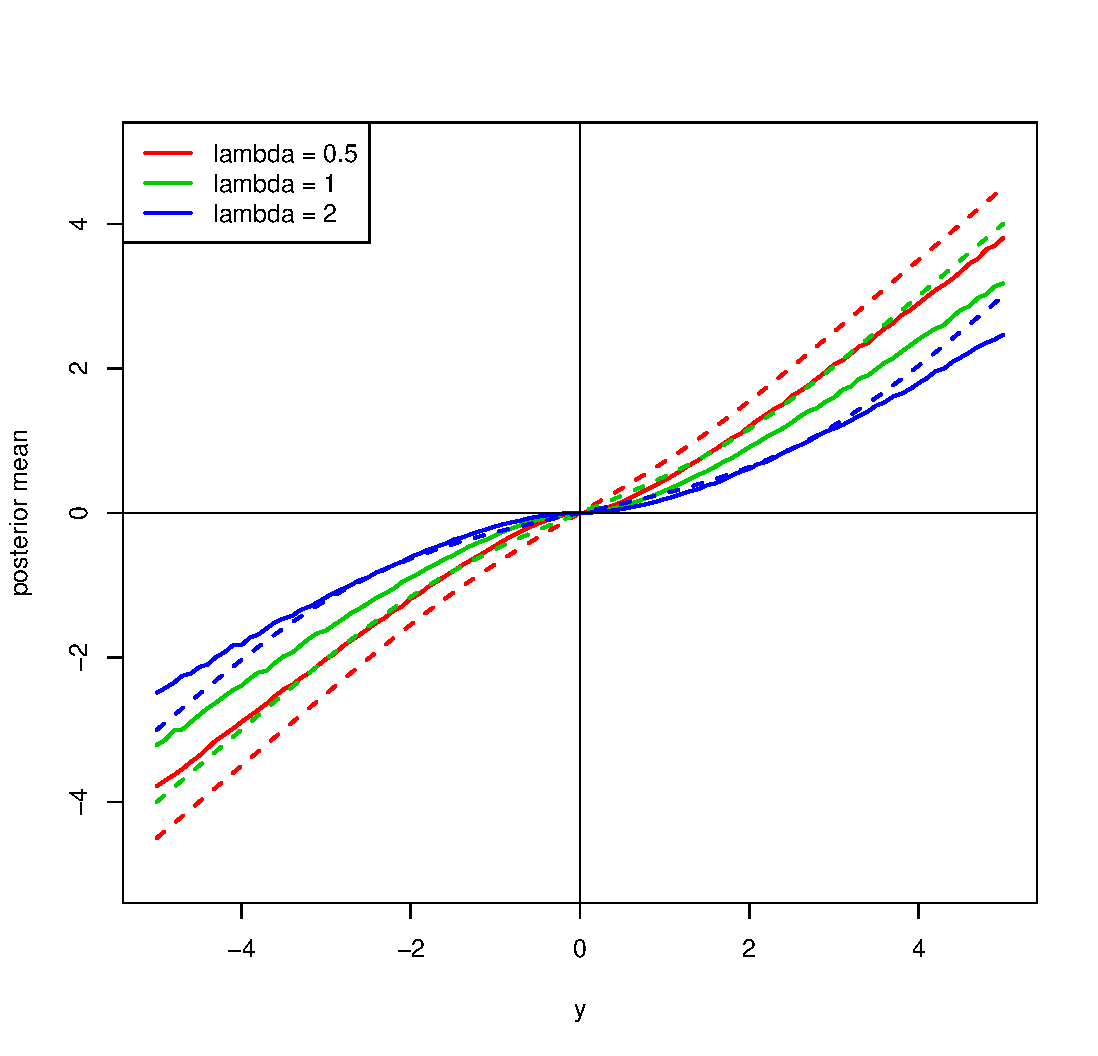
\includegraphics[scale=0.55]{simple.pdf} 
\caption{Normal means model with LASSO prior: WBB mean $E_{{\bf w}}(\theta^*_{\bf w}|y)$ (in solid lines) versus exact posterior mean $E(\theta|y)$ (in dashed lines).}
\label{simple}
\end{figure}
The WBB mean $E_{{\bf w}}(\theta^*_{\bf w}|y)$ is approximated by the sample mean of $\{ \theta^{*,t}_{\bf w}\}_{t=1}^T$. On the other hand, Mitchell (1994) gives the expression for the posterior mean, 
\begin{eqnarray*}
E(\theta|y) &=& \frac{\int_{-\infty}^\infty \theta\exp\left\{-(y-\theta)^2/2 - \lambda |\theta|\right\} d\theta}{\int_{-\infty}^\infty \exp\left\{-(y-\theta)^2/2 - \lambda |\theta|\right\} d\theta}\\
&=& \frac{F(y)}{F(y) + F(-y)}(y+\lambda) + \frac{F(-y)}{F(y) + F(-y)}(y-\lambda)\\
&=& y + \frac{F(y) - F(-y)}{F(y) + F(-y)}\lambda
\end{eqnarray*}
where $F(y) = \exp(y)\Phi(-y-\lambda)$ and $\Phi(\cdot)$ is the c.d.f. of standard normal distribution. We plot  the WBB mean versus the exact posterior mean in Figure (\ref{simple}).  Interestingly, the WBB algorithm shrinks the posterior means towards zero. 
WBB samples are approximate posterior draws, though the algorithm structure does not
permit a clear descripton of the prior that is in force for this sampled distribution.
Whatever is this  effective prior, it may be different from the prior encoded in the
penalty used in repeated optimization, as the result in Figure~(1) suggests.


A simulation study is conducted in order to further investigate WBB in the context of regression. 
We simulate data from the linear model,
$$
y = X\beta + \epsilon, \; \epsilon \sim N(0, \sigma_\epsilon^2 I)
$$
where $X$ is $n\times p$ and $y$ is $n\times 1$. The design matrix $X$ 
is generated by drawing its $n$ rows independently from 
a $p$-dimensional normal distribution, $N({\bf 0}, \Sigma)$. Within each row, the covariance 
between entries in columns $i$ and $j$ is set to be $\Sigma_{i,j} = 0.1\times 0.8^{|i-j|}$. Further we set the noise variance $\sigma_\epsilon^2 = \Vert X\beta \Vert^2_2/(2n)$. In this setting, the signal-to-noise ratio is 2. 
 Figure (\ref{mcmc}) displays WBB samples (kernel density
estimates) and posteriors via MCMC in one of the simulation settings;
$n=50, p=2, \sigma_\epsilon^2=1, \Sigma = [[1, 0.3]', [0.3,1]']$ and $\beta_1 = 0, \beta_2 = 2$.
The WBB (on the $L^1$, LASSO prior penalty) is compared  to  posteriors computed via MCMC under
several different priors: the same $L^1$ prior encoded in the WBB penalty, and also
two $L^0$ penalties,  $p(\beta) \propto \exp\{-\lambda \Vert \beta\Vert_0\}$ and $p(\beta) \propto \exp\{-5\lambda \Vert \beta\Vert_0\}$ (Polson and Sun, 2019).
The WBB samples entail a spike at $\beta_1 = 0$, indicating a positive probability mass in the
effective prior. No such posterior mass is evident in the $L^0$ priors nor possible in
 the $L^1$ prior.

\begin{figure}[!ht]
\centering
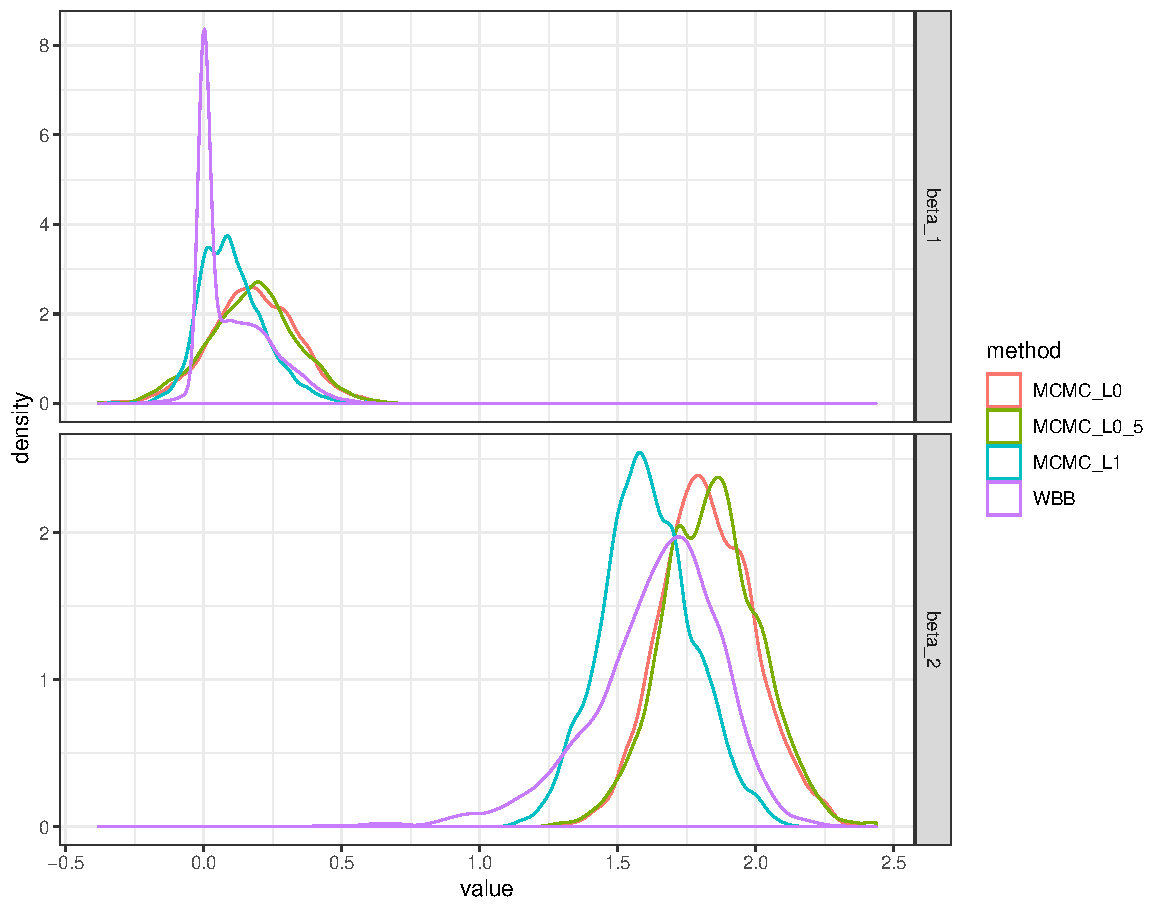
\includegraphics[scale=0.55]{mcmc}
\caption{WBB samples under LASSO penalty, compared with posteriors under  LASSO prior and $L^0$ prior computed by MCMC.}
\label{mcmc}
\end{figure}


Next we use the simulation to compare WBB distributions to MCMC-computed posteriors in a range of regression
settings.
We consider both sparse and dense cases for the coefficient vector $\beta = [\beta_1, \beta_2, ..., \beta_p]'$:
\begin{enumerate}
	\item[A(i).] $\beta_j = 1$ for $1 \leq j \leq 10$ and $\beta_j = 0$ for $j > 10$.
	\item[A(ii).] $\beta_j = 1$ for $1 \leq j \leq 5$, $\beta_j = 10$ for $6 \leq j \leq 10$ and $\beta_j = 0$ for $j > 10$.
	\item[B.] $\beta_j = 1$ for $1 \leq j \leq p$.
\end{enumerate}
For each setting of $\beta$, we consider $p = 40, 60, 80, 100, 120$. To investigate the performance of WBB under different sample sizes, we also choose two settings of $n$: $n=100$ for all $p$, or $n=p/2$ for all $p$.

We compare the WBB with LASSO prior and separate weights to Markov chain Monte Carlo under
the Bayesian LASSO (Park and Casella, 2008; Carlin and Polson, 1991). 
 The two methods entail different prior penalties: 
\begin{eqnarray*}
\text{WBB}:& \; \lambda\phi(\beta | {\bf w}) = \lambda \sum_{j=1}^p w_{0,j} |\beta_j|,\\
\text{BLASSO}:& \; \phi(\beta | \sigma^2) = -\log\left(\frac{\lambda}{2\sigma}\right) + \frac{\lambda}{\sigma} \sum_{j=1}^p  |\beta_j|.
\end{eqnarray*}
Bayesian LASSO imposes a noninformative marginal prior on $\sigma^2$, $\pi(\sigma^2) = 1/\sigma^2$ and the posterior distribution is sampled by a Gibbs sampler, with $\lambda$ chosen by maximizing the marginal likelihood. In WBB, $\lambda$ is chosen via cross-validation, using standard unweighted LASSO. Here the original LASSO prior is separable 
and we study the separate-weights version of WBB.
 In high-dimensional cases, a large common $w_0$ multiplied to $\phi(\beta)$ can introduce extra sparsity to all marginal posteriors.  We use separate weights in an effort to overcome this issue. 
For comparison criteria, we present the estimation MSE of coefficients $\beta$ (use posterior mean as our estimate), out-of-sample prediction MSE (test sets are of the same size as the corresponding training sets), and the mean of the 95\% credible interval coverages. Fixing $(p, n, \beta)$,  we draw $T=200$ posterior samples by each method and the estimation procedure is repeated over $B=500$ independent datasets $\{(X,y)^{(b)}\}_{b=1}^B$. Let $\beta^{*,t}(b)$ denote the $t$-th posterior draw, with respect to the $b$-th dataset. For each coordinate $j$,  coverage is calculated using $\{\beta_j^{*,t}(b): 1\leq t \leq T, 1\leq b \leq B\}$. The coverages are then averaged across $1\leq j \leq p$. 

%To further understand how the two methods compare on the structure of the posterior, we define the model-selection discrepancy as 
%$$
%d(\beta^*, \beta) = \frac{1}{p} \sum_{j=1}^p \left( \mathds{1}\{\beta_{j}^*=0, \beta_{j}\neq 0\} + \mathds{1}\{\beta_{j}^*\neq 0, \beta_{j}=0\} \right)
%$$
%where $\beta^*$ is a draw from the posterior distribution produced by WBB or Bayesian LASSO. 
%The mean model-selection discrepancy  is then estimated by averaging $d(\beta^*,\beta)$ over both posterior
%samples and simulated data sets.
%%$$
%\hat E\left[d(\beta^*, \beta) | y\right] = \frac{1}{pT} \sum_{t=1}^T\sum_{j=1}^p \mathds{1}\{\beta_{j}^{*,t}=0, \beta_{j}\neq 0\} + \mathds{1}\{\beta_{j}^{*,t}\neq 0, \beta_{j}=0\}.
%$$
%Note that we will further average it over $B$ datasets.


\renewcommand{\arraystretch}{0.5}
\begin{table}[ht]\label{beta-mse}
	\tbl{Coefficient Estimation Mean Squared Error (MSE)}{%
\begin{tabular*}{30pc}{@{\hskip5pt}@{\extracolsep{\fill}}c@{}c@{}c@{}c@{}c@{}c@{}c@{}c@{}@{\hskip5pt}}
\toprule
	&                     & $p$      & 40   & 60   & 80   & 100  & 120  \\ \colrule
		\multirow{6}{*}{$n = 50$}  & \multirow{2}{*}{A(i)}  & BLASSO & 0.13 & 0.09 & 0.06 & 0.05 & 0.04 \\
               &       & WBB    & 0.19 & 0.06 & 0.05 & 0.04 & 0.03 \\
		& \multirow{2}{*}{A(ii)} & BLASSO & 5.59 & 3.74 & 2.90 & 2.33 & 1.96 \\
               &       & WBB    & 7.40 & 2.89 & 2.31 & 1.90 & 1.62 \\
		& \multirow{2}{*}{B}     & BLASSO & 0.67 & 0.67 & 0.68 & 0.70 & 0.70 \\
               &       & WBB    & 1.77 & 0.49 & 0.50 & 0.51 & 0.52 \\  \colrule
		\multirow{6}{*}{$n = p/2$} & \multirow{2}{*}{A(i)}  & BLASSO & 0.13 & 0.08 & 0.06 & - & 0.05 \\
               &       & WBB    & 0.14 & 0.08 & 0.05 & - & 0.03 \\ 
		& \multirow{2}{*}{A(ii)} & BLASSO & 6.88 & 4.09 & 2.88 & - & 1.94 \\
               &       & WBB    & 6.58 & 3.80 & 2.53 & - & 1.47 \\ 
		& \multirow{2}{*}{B}     & BLASSO & 0.52 & 0.56 & 0.64 & - & 0.74 \\
               &       & WBB    & 0.68 & 0.62 & 0.55 & - & 0.48 \\ \botrule
\end{tabular*}}
\end{table}	
	
		
\begin{table}[ht]
	\label{oos-mse}
	\tbl{Out-of-Sample Prediction Mean Squared Error (MSE)}{%
\begin{tabular*}{30pc}{@{\hskip5pt}@{\extracolsep{\fill}}c@{}c@{}c@{}c@{}c@{}c@{}c@{}c@{}@{\hskip5pt}}
\toprule
	&                     & $p$      & 40   & 60   & 80   & 100  & 120  \\ \colrule	
		\multirow{6}{*}{$n = 50$}  & \multirow{2}{*}{A(i)}  & BLASSO & 3.35   & 3.42   & 3.43   & 3.61   & 3.68   \\
               &       & WBB    & 3.34   & 3.37   & 3.40   & 3.60   & 3.72   \\
		& \multirow{2}{*}{A(ii)} & BLASSO & 119.65 & 124.03 & 130.49 & 132.21 & 135.46 \\
               &       & WBB    & 121.45 & 123.40 & 129.89 & 134.04 & 140.44 \\
		& \multirow{2}{*}{B}     & BLASSO & 20.24  & 33.18  & 46.75  & 61.86  & 80.57  \\
               &       & WBB    & 20.61  & 32.47  & 46.27  & 60.59  & 78.71  \\  \colrule
		\multirow{6}{*}{$n = p/2$} &  \multirow{2}{*}{A(i)} & BLASSO & 4.55   & 4.15   & 3.83   & -      & 3.61   \\
               &       & WBB    & 3.65   & 3.75   & 3.66   & -      & 3.65   \\
		& \multirow{2}{*}{A(ii)}  & BLASSO & 180.56 & 153.56 & 136.82 & -      & 128.39 \\
               &       & WBB    & 145.73 & 141.35 & 133.66 & -      & 132.23 \\
		& \multirow{2}{*}{B}      & BLASSO & 26.35  & 39.23  & 50.77  & -      & 73.63  \\
               &       & WBB    & 21.80  & 34.82  & 47.76  & -      & 75.29  \\ \botrule
	\end{tabular*}}
\end{table}


\begin{table}[ht]
	\label{tab:coverage}
	\tbl{95\% Credible Interval Coverage}{%
\begin{tabular*}{30pc}{@{\hskip5pt}@{\extracolsep{\fill}}c@{}c@{}c@{}c@{}c@{}c@{}c@{}c@{}@{\hskip5pt}}
\toprule
	&                        & $p$      & 40   & 60   & 80   & 100  & 120  \\ \colrule
		\multirow{6}{*}{$n = 50$}  & \multirow{2}{*}{A(i)}  & BLASSO & 0.91   & 0.92   & 0.93   & 0.94   & 0.94   \\
               &       & WBB    & 0.92   & 0.92   & 0.93   & 0.94   & 0.95   \\
		& \multirow{2}{*}{A(ii)}  & BLASSO & 0.91   & 0.93   & 0.95   & 0.96   & 0.96   \\
               &       & WBB    & 0.91   & 0.92   & 0.94   & 0.94   & 0.95   \\
		& \multirow{2}{*}{B}     & BLASSO & 1.00   & 1.00   & 1.00   & 1.00   & 1.00   \\
               &       & WBB    & 0.95   & 0.96   & 0.94   & 0.93   & 0.91   \\ \colrule
		\multirow{6}{*}{$n = p/2$} & \multirow{2}{*}{A(i)}  & BLASSO & 0.93   & 0.93   & 0.94   & -      & 0.94   \\
               &       & WBB    & 0.91   & 0.92   & 0.93   & -      & 0.94   \\
		& \multirow{2}{*}{A(ii)} & BLASSO & 0.92   & 0.94   & 0.95   & -      & 0.96   \\
               &       & WBB    & 0.91   & 0.93   & 0.94   & -      & 0.95   \\
		& \multirow{2}{*}{B}     & BLASSO & 1.00   & 1.00   & 1.00   & -      & 1.00   \\
               &       & WBB    & 0.94   & 0.93   & 0.93   & -      & 0.92   \\  \botrule
	\end{tabular*}}
\end{table}


%\begin{table}[ht]
%	\label{tab:discrepancy}
%	\tbl{Mean Model-selection Discrepancy}{%
%\begin{tabular*}{30pc}{@{\hskip5pt}@{\extracolsep{\fill}}c@{}c@{}c@{}c@{}c@{}c@{}c@{}c@{}@{\hskip5pt}}
%\toprule
%	&                        & $p$      & 40   & 60   & 80   & 100  & 120  \\ \colrule
%		\multirow{6}{*}{$n = 50$}  & \multirow{2}{*}{A(i)}  & BLASSO & 0.44   & 0.46   & 0.46   & 0.43   & 0.38   \\
%               &       & WBB    & 0.38   & 0.26   & 0.22   & 0.19   & 0.17   \\
%		& \multirow{2}{*}{A(ii)}  & BLASSO & 0.45   & 0.46   & 0.47   & 0.44   & 0.39   \\
%               &       & WBB    & 0.38   & 0.26   & 0.22   & 0.19   & 0.17   \\
%		& \multirow{2}{*}{B}     & BLASSO & 0.46   & 0.48   & 0.49   & 0.54   & 0.60   \\
%               &       & WBB    & 0.55   & 0.80   & 0.83   & 0.85   & 0.87   \\\colrule
%		\multirow{6}{*}{$n = p/2$} & \multirow{2}{*}{A(i)}  & BLASSO & 0.44   & 0.43   & 0.43   & -      & 0.44   \\
%               &       & WBB    & 0.31   & 0.25   & 0.21   & -      & 0.17   \\
%		& \multirow{2}{*}{A(ii)} & BLASSO & 0.44   & 0.43   & 0.43   & -      & 0.44   \\
%               &       & WBB    & 0.31   & 0.25   & 0.22   & -      & 0.17   \\
%		& \multirow{2}{*}{B}     & BLASSO & 0.57   & 0.55   & 0.54   & -      & 0.54   \\
%               &       & WBB    & 0.81   & 0.82   & 0.84   & -      & 0.86    \\  \botrule
%	\end{tabular*}}
%\end{table}

The complete results for estimation error,  out-of-sample prediction error, and credible interval coverage are displayed in Table (1), (2), and (3), respectively. In almost all cases when $p\geq 60$, WBB has lower estimation error than BLASSO. 
WBB shows comparable or superior out-of-sample prediction in most cases. 
 Credible intervals of neither WBB nor BLASSO have exact 95\% coverage.  WBB performs well when $p \geq 100$ and $\beta$ is sparse, though it often under covers.  When $\beta_j = 1$ for all $1 \leq j \leq p$, BLASSO intervals are too wide while WBB intervals have coverage close to 95\% when $40 \leq p \leq 80$.    Though limited in scope, this simulation reveals some distinctions
and also  broad similarities between WBB and Bayesian LASSO in both posterior structure and the sampling performance of approximate posterior summaries. It may provide
a useful basis for further methodological development.  Serial computations were used in the simulation above, and
WBB was  slightly slower than BLASSO  (by a factor of 1.5 on CPU time);  the computational advantage of WBB shows up in
parallel computations, since weight vectors induce separate optimizations. 

\subsection{Diabetes Data}
To further illustrate the WBB methodology, we apply it to the often-analyzed diabetes dataset (Efron {\em et al.}, 2004). The measurements for 442 diabetes patients are obtained ($n=442$), with 10 baseline variables ($p=10$), including age, sex, body mass index, average blood pressure, and six blood serum measurements. 

%The likelihood function is given by
%$$
%l(y|\beta) = \prod_{i=1}^n p(y_i|\beta)
%$$
%where
%$$
%p(y_i|\beta) = \frac{1}{\sqrt{2\pi}\sigma} \exp\left\{-\frac{1}{2\sigma^2}(y_i - x_i'\beta)^2 \right\}.
%$$

\noindent We draw 1000 sets of weights as i.i.d. exponentials as in Algorithm~1. For each weight set, the weighted Bayesian estimate $\beta^*_{\bf w}$ is calculated using Equation (\ref{eqn:diabetes}) via the regularization method in the package {\tt glmnet}. 

\begin{equation}
\label{eqn:diabetes}
\beta^{*,{\rm common}}_{\bf w} := \underset{\beta}{\argmin} \;\sum_{i=1}^n w_i(y_i - x_i'\beta)^2+ \lambda w_{0}\sum_{j=1}^p |\beta_j|\; . 
\end{equation}
The regularization factor $\lambda$ is chosen by cross-validation with unweighted likelihood. The WBB is also performed with separate weights on each $|\beta_j|$,
\begin{eqnarray*}}
\beta^{*,{\rm separate}}_{\bf w} := \underset{\beta}{\argmin} \;\sum_{i=1}^n w_i(y_i - x_i'\beta)^2+ \lambda \sum_{j=1}^p w_{0,j} |\beta_j|\; . 
\end{eqnarray*}}
As in the simulation study, WBB results are compared with the Bayesian LASSO. 
\begin{figure}[!ht]
\centering 
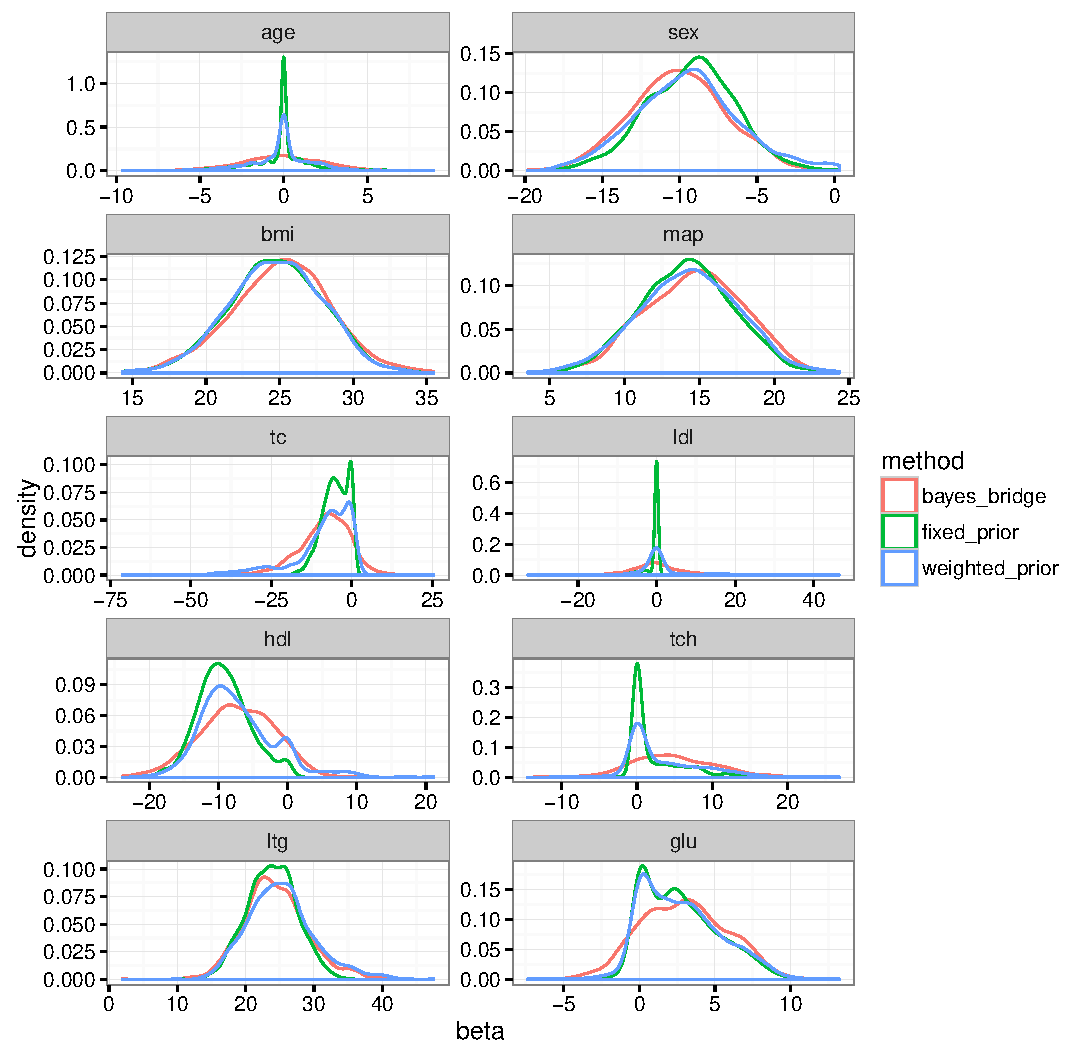
\includegraphics[scale=0.7]{diabetes.pdf} 
\caption{Diabetes example: the weighted Bayesian Bootstrap (with common prior weight
(blue) and separate prior weights (green)) and Bayesian LASSO (red) are used to draw from the marginal posteriors for $\beta_j$'s, j = 1,2,...10. }
\label{diabetes}
\end{figure}

Figure (\ref{diabetes}) shows the results of all these three methods (the WBB with common/separate  weight on prior terms , and Bayesian LASSO). Marginal posteriors for $\beta_j$'s are presented. 
For some coefficients there is very good agreement among the methods (e.g. {\tt bmi} and {\tt map}).
 One notable feature is that the WBB tends to introduce less sparsity than Bayesian LASSO. For example, the Bayesian LASSO posteriors of {\tt age, tc, ldl, tch} and {\tt glu} have higher spikes near zero compared with the WBB.

%For {\tt tc} and {\tt hdl}, multi-modes in the marginal posteriors are observed. In general, the posteriors with 
%separate weights on prior terms are similar with those given common prior weight. This difference is naturally attributed to variation in the weight assigned to the log-prior penalty term. 

\subsection{Trend Filtering}
The generalized LASSO solves the optimization problem:
\begin{eqnarray*}
\beta^* &=& \underset{\beta}{\argmin} \, \left\{ l(y|\beta) + \lambda\phi(\beta)  \right\}\\
&=& \underset{\beta}{\argmin} \, \frac{1}{2}\|y - X\beta\|_2^2 + \lambda \|D\beta\|_1
\end{eqnarray*}
where $ l(y|\beta) = \frac{1}{2}\|y - X\beta\|_2^2 $ is the negative log-likelihood. $D \in \R^{m\times p}$ is a penalty matrix and $ \lambda\phi(\beta) = \lambda \|D\beta\|_1$ is the negative log-prior or regularization penalty. There are fast path algorithms for solving this problem (see {\tt genlasso} package).

As a subproblem, polynomial trend filtering (Tibshirani, 2014; Polson and Scott, 2015) allows for piece-wise polynomial curve-fitting, where the knots and the parameters are chosen adaptively. Intuitively, the trend-filtering estimator is similar to an adaptive spline model: it penalizes the discrete derivative of order $k$, resulting in piecewise polynomials of higher degree for larger $k$.

\begin{figure}[ht]
\centering 
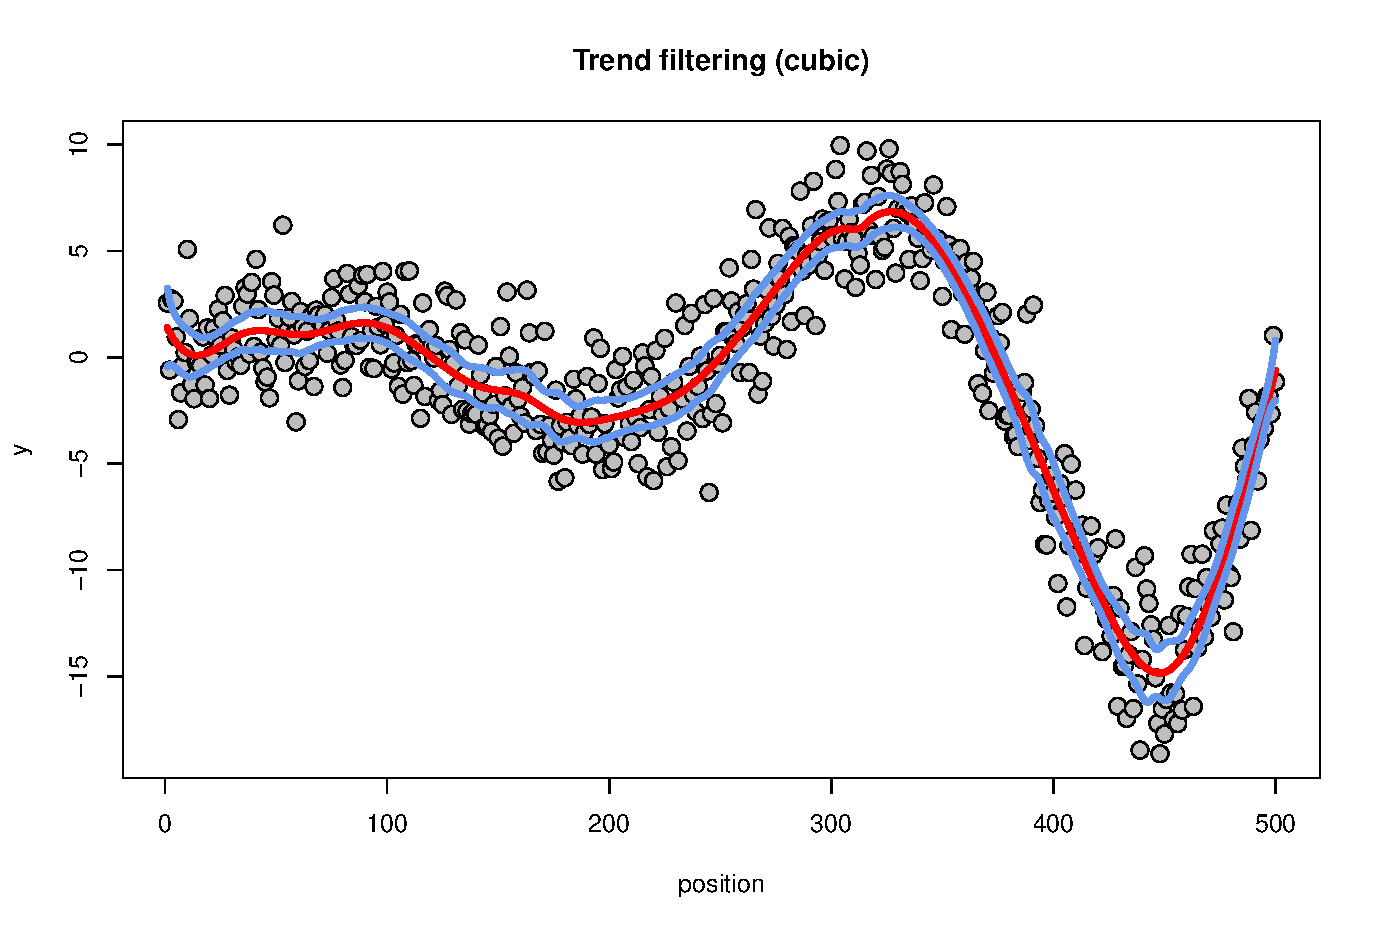
\includegraphics[scale=0.55]{filtering.pdf} 
\caption{Cubic trend filtering: the red line is $\hat\beta_i$ for $i=1,2,...500$; the blue line is $\hat\beta_i \pm 2*se$ where the standard errors are computed by WBB. $\lambda = 1000$.}
\label{filter}
\end{figure}

Specifically, $X = I_p$ in the trend filtering setting  and the data $y = (y_1, ..., y_p)$ are assumed to be meaningfully ordered from 1 to $p$. The penalty matrix is specially designed by the discrete $(k+1)$-th order  derivative,
$$D^{(1)}=
\begin{bmatrix}
    -1       & 1 & 0 & \dots & 0 & 0 \\
    0       & -1 & 1 & \dots & 0 & 0 \\
    \hdotsfor{5} \\
    0       & 0 & 0 & \dots & -1 & 1
\end{bmatrix}_{(p-1)\times p}
$$
and $D^{(k+1)} = D^{(1)}D^{(k)}$ for $k =1,2,3...$. For example, the log-prior in linear trend filtering is explicitly written as $\lambda\sum_{i=1}^{p-2}|\beta_{i+2} - 2\beta_{i+1} + \beta_{i}|$. For a general order $k >1$, 
$$
\|D^{(k+1)}\beta\|_1 = \sum_{i=1}^{p-k-1} \Big| \sum_{j=i}^{i+k+1} (-1)^{(j-i)} \binom{k+1}{j-i}\beta_j \Big|.
$$
WBB solves the following generalized LASSO problem in each draw:
\begin{eqnarray*}
 \beta_{\bf w}^* &=& \underset{\beta}{\argmin} \, \frac{1}{2}\sum_{i=1}^p w_i(y_i - \beta_i)^2 + \lambda w_{0}\|D^{(k)}\beta\|_1\\
&=&\underset{\beta}{\argmin} \, \frac{1}{2}  \|Wy - W\beta\|_2^2  + \lambda \|D^{(k)}\beta\|_1\\
&=&W^{-1}  \underset{\tilde\beta}{\argmin} \, \frac{1}{2}  \|\tilde{y}_{\bf w} - \tilde{\beta}_{\bf w}\|_2^2  + \lambda \|\tilde{D}^{(k)}_{\bf w}\tilde{\beta}_{\bf w}\|_1
\end{eqnarray*}where 
$W = {\rm diag}\left(\sqrt{w_1},\cdots,  \sqrt{w_p}\right)/\sqrt{w_{0}}$ and $$\tilde{y}_{\bf w} = Wy, \, \tilde{\beta}_{\bf w} = W\beta, \,   \tilde{D}^{(k)}_{\bf w}= D^{(k)}W^{-1}.$$
To illustrate, we simulate data $y_i$ from a Fourier series regression 
$$
y_i = \sin\left(\frac{4\pi}{500} i\right)\exp\left({\frac{3}{500} i}\right) + \epsilon_i
$$
for $i=1,2, \cdots, n=500$, where $\epsilon_i\sim N(0,2^2)$ are i.i.d. Gaussian deviates. The cubic trend filtering result is given in Figure (\ref{filter}). 
For each $i$, the WBB gives a group of estimates $\left\{\beta_{\bf w}^{*, t}(i) \right\}_{t=1}^T$ where $T$ is the total number of draws. The standard deviation of these weighted solutions constitutes a posterior standard deviation, or
essentially  a standard error for the estimator $\hat \beta_i$.
\subsection{Deep Learning: MNIST Example}
Deep learning is a form of machine learning that uses hierarchical abstract layers of latent variables to perform pattern matching and prediction.  A Bayesian probabilistic perspective provides a number of insights into more efficient algorithms for optimization
and hyper-parameter tuning.  The general goal is to find a predictor of an output $y$ given a high dimensional input $x$. For a classification problem, $y \in \{1, 2, ..., K\}$ is a discrete variable and can be coded as a $K$-dimensional 0-1 vector. The model is as follows. Let $z^{(l)}$ denote the $l$-th layer, and so $x = z^{(0)}$. The final output is the response $y$,
which can be numeric or categorical. A deep prediction rule (Polson and Sokolov, 2017) is then 
\begin{align*}
z^{(1)} & = f^{(1)} \Big( W^{(0)} x + b^{(0)} \Big),\\
z^{(2)} & = f^{(2)} \Big( W^{(1)} z^{(1)} + b^{(1)} \Big),\\
& \cdots \\
z^{(L)} & = f^{(L)} \Big( W^{(L-1)} z^{(L-1)} + b^{(L-1)} \Big),\\
\hat{y} (x) & = z^{(L)}.
\end{align*}
Here, $W^{(l)}$ are weight matrices, and $b^{(l)}$ are threshold or activation levels. $f^{(l)}$ is the activation function. Probabilistically, the output $y$ in a classification problem is generated by a probability model 
$$
p(y|x, W, b) \propto \exp\{-l(y|x, W, b)\}
$$
where $l(y|x, W, b) = \sum_{i=1}^{n}l_i(y_i|x_i, W, b) $ is the  negative cross-entropy,
$$
l_i(y_i|x_i, W, b) = l_i(y_i, \hat{y}(x_i)) = \sum_{k=1}^K y_{ik}\log\hat{y}_k(x_i)
$$
where $y_{ik}$ is 0 or 1.
Adding the negative log-prior $\lambda\phi(W, b)$, the objective function (negative log-posterior) to be minimized by stochastic gradient descent is 
$$
\mathcal{L}_\lambda(y,\hat{y}) = \sum_{i=1}^{n}l_i(y_i, \hat{y}(x_i)) + \lambda\phi(W, b).
$$
Accordingly, with each draw of weights ${\bf w}$, WBB provides the estimates $(W^*_{\bf w}, b^*_{\bf w})$ by solving the following optimization problem:
$$
(W^*_{\bf w}, b^*_{\bf w}) = \argmin_{W, b} \sum_{i=1}^{n}w_i l_i(y_i|x_i, W, b) + \lambda w_0\phi(W, b).
$$
We take the classic MNIST example (LeCun and Cortes, 2010) to illustrate the application of WBB in deep learning. The MNIST database of handwritten digits, available from Yann LeCun's website, has 60,000 training examples and 10,000 test examples. Here the high-dimensional $x$ is a normalized and centered fixed-size ($28\times 28$) image and the output $\hat{y}$ is a 10-dimensional vector, where $i$-th coordinate corresponds to the probability of that image being the $i$-th digit.

For simplicity, we build a 2-layer neural network with layer sizes 128 and 64 respectively. Therefore, the dimensions of parameters are
\begin{align*}
W^{(0)} \in \R^{128\times 784},\, b^{(0)}\in \R^{128},\\
W^{(1)} \in \R^{64\times 128},\, b^{(1)}\in \R^{64},\\
W^{(2)} \in \R^{10\times 64},\, b^{(0)}\in \R^{10}.
\end{align*}
The activation function $f^{(i)}$ is ReLU, $f(x) = \max\{0,x\}$, and the negative log-prior is specified as 
$$
\lambda\phi(W,b) = \lambda\sum_{l=0}^{2}\Vert W^{(l)} \Vert_2^2
$$
where we manually set $\lambda = 10^{-4}$. 
\begin{figure}[!ht]
	\centering
	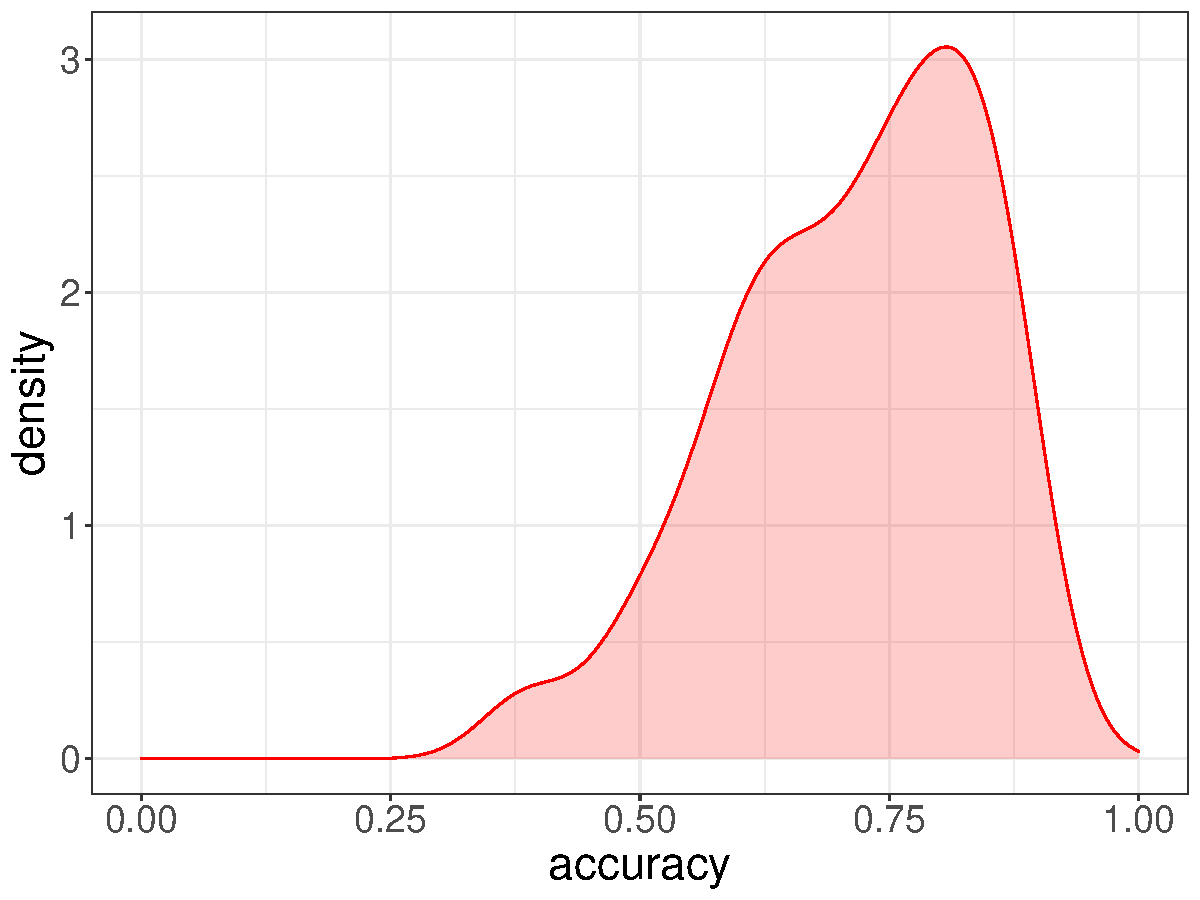
\includegraphics[width=0.7\linewidth]{acc}
	\caption{Posterior distribution of the classification accuracy. $n=500, \lambda=10^{-4}$.}
	\label{fig:acc}
\end{figure}
Figure (\ref{fig:acc}) shows the posterior distribution of the classification accuracy in the test dataset. We see that the test accuracies are centered around 0.75 and the posterior distribution is left-skewed. Furthermore, the accuracy is higher than 0.35 in 99\% of the cases. The 95\% interval is [0.407, 0.893].  Due to the simple 2-layer neural network structure, the classification accuracy is admittedly low compared with the state-of-the-art (e.g., Liang and Hu,  2015). This illustrative example shows how WBB can be easily implemented in deep learning. Implementing Variational Bayes in deep learning is discussed in Polson and Sokolov (2017).

\section{Discussion}
Weighted Bayesian Bootstrap (WBB) provides a computationally attractive solution to scalable Bayesian inference (Minsker {\em et al.}, 2014; Welling and Teh, 2011)
whilst accounting for parameter uncertainty by maximizing a weighted posterior distribution. WBB can also be used in conjunction with proximal methods (Parikh and Boyd, 2013; Polson {\em et al.}, 2015)
to provide  sparsity in high dimensional statistical problems. With a similar ease of computation, WBB provides an alternative to approximate Bayesian computation (ABC)
 methods (Beaumont, 2009) and variational Bayes (VB) methods. (See Blei {\em et al}, 2017, for a review of variational inference in Bayesian statistics.) A fruitful area for future research is the comparison of WBB to recent extensions of 
the weighted likelihood bootstrap for generalized Bayesian inference 
(Lyddon {\em et al.}, 2019).


For a wide range of non-smooth objective functions/statistical models, recent regularization methods provide fast, scalable algorithms for calculating estimates of the form (\ref{eqn:canonicalform}), which can also be viewed as posterior modes. Therefore as $\lambda$ varies we obtain a full regularization path as a form of prior sensitivity analysis. Further, Strawderman {\em et al.} (2013) and Polson and Scott (2015) 
considered scenarios where posterior modes can be used as posterior means from augmented probability models.
There may be useful interpretations of the random weights from the data-augmentation perspective.


Extending WBB asymptotics presents an exciting research opportunity.   
The argument in Section 2.5 
relies on smoothness in both the sampling model and prior, and it retains fixed parameter
dimension as $n$ increases.  Theoretical guarantees remain unavailable for relatively large parameter
dimension or for non-smooth penalty functions.  Fortunately, groundwork has been done, for example by 
Van Der Pas {\em et al.}, (2014), Narisety and  He  (2014), and others on the asymptotic  behaviour of the 
posterior distribution,  and by Knight and Fu (2000) and others on sampling theory of 
optimization-based estimators,



%{\em **Nick, not sure where this should go.**
%A general class of natural exponential family models can be expressed in terms of the Bregman divergence of the dual of the cumulant transform.
%Let $ \phi $ be the conjugate Legendre transform of $\psi$. Hence $ \psi(\theta) = \sup_\mu \; \left ( \mu^\top \theta - \phi(\mu) \right )$. Then we can write
%\begin{align*}
%p_\psi ( y | \theta ) & = \exp \left ( y^\top \theta - \psi( \theta) - h_\psi(y) \right )\\
% & = \exp \left \{ \inf_\mu \; \left ( ( y - \mu )^\top \theta - \phi(\mu) \right ) - h_\psi(y) \right \}\\
%& = \exp \left ( - D_\phi ( y , \mu(\theta) ) - h_\phi (y) \right )
%\end{align*}
%where the infimum is attained at $ \mu(\theta) = \phi^\prime (\theta) $ is the mean of the exponential family distribution.
%We rewrite $ h_\psi(y) $ is terms of the correction term and $ h_\phi(y)$. Here there is a duality as $D_\phi$ can be interpreted as a Bregman divergence.}



\begin{thebibliography}{}

\bibitem[Abadi et al., 2015]{tensorflow2015-whitepaper}
Abadi, M., Agarwal, A., Barham, P., Brevdo, E., Chen, Z., Citro, C., Corrado, G. S., Davis, A., Dean, J., Devin, M., Ghemawat, S., Goodfellow, I., Harp, A., Irving, G., Isard, M., Jia, Y., Jozefowicz, R., Kaiser, L., Kudlur, M., Levenberg, J., Man\'{e}, D., Monga, R., Moore, S., Murray, D., Olah, C., Schuster, M., Shlens, J., Steiner, B., Sutskever, I., Talwar, K., Tucker, P., Vanhoucke, V., Vasudevan, V., Vi\'{e}gas, F., Vinyals, O., Warden, P., Wattenberg, M., Wicke, M., Yu, Y., \& Zheng, X. (2015) TensorFlow: Large-scale machine learning on heterogeneous systems. {\it Software available from tensorflow.org}.

\bibitem[Arnold \& Tibshirani, 2014]{arnold2014genlasso}
Arnold, T. B., and Tibshirani, R. J. (2014). genlasso: Path algorithm for generalized lasso problems. {\it R package version 1.3}.

\bibitem[BB12]{bb12}
Barbe, P. and Bertail, P. (2012). {\em The weighted bootstrap} Vol. 98. Springer Science \& Business Media.

\bibitem[Beaumont et al., 2009]{beaumont2009adaptive}
Beaumont, M. A.,  Cornuet, J.M.,  Marin,J.M. and Robert, C. P. (2009). Adaptive approximate Bayesian computation. {\it Biometrika}, 96(4), 983--990.

\bibitem[Blei et al., 2017]{blei2017variational}
Blei, D. M., Kucukelbir, A., and  McAuliffe, J. D. (2017). Variational inference: A review for statisticians. {\it Journal of the American Statistical Association}, 112(518), 859-877.

\bibitem[Bertail \& Lo, 1991]{Bertail}
Bertail, P. and Lo,  A. Y.  (1991). On Johnson's asymptotic expansion for a posterior distribution. {\it Centre de Recherche en Economie et Statistique}.

\bibitem[Bertsekas et al. 2003]{bertsekas2003}
Bertsekas, D.P., Nedi, A. and Ozdaglar, A.E. (2003). {\em Convex analysis and optimization}. Athena Scientific.

\bibitem[Boyd \& Vandenberghe, 2004]{boyd2004convex}
Boyd, S. and Vandenberghe, L. (2004) {\it Convex optimization}. Cambridge university press.

\bibitem[Carlin \& Polson, 1991]{carlin1991inference}
Carlin, B. P., and Polson, N. G. (1991). Inference for nonconjugate Bayesian models using the Gibbs sampler. {\it Canadian Journal of statistics}, 19(4), 399-405.

\bibitem[Chollet et al., 2015]{chollet2015keras}
Chollet, Fran\c{c}ois and others. (2015) Keras {\it https://keras.io}

\bibitem[Efron et al., 2004]{efron2004least}
Efron, B., Hastie, T., Johnstone, I. \& Tibshirani, R. J. (2004).  Diabetes dataset. Available from R package {\it lars}.

\bibitem[Friedman{,} Hastie \& Tibshirani, 2010]{friedman2010regularization} 
Friedman, J.,  Hastie, T. and  Tibshirani, R. J. (2010). Regularization Paths for Generalized Linear Models via Coordinate Descent. {\it Journal of Statistical Software}, 33(1),1--22.

\bibitem[Gelman \& Meng, 1998]{gelman1998simulating}
Gelman, A. and Meng, X.L. (1998). Simulating normalizing constants: From importance sampling to bridge sampling to path sampling. {\it Statistical Science}, 163--185.

\bibitem[Gordon{,}  Salmond \& Smith, 1993]{gordon1993novel}
Gordon, N. J.,  Salmond, D. J. and  Smith, A. F. (1993). Novel approach to nonlinear/non- gaussian Bayesian state estimation. {\it In IEE Proceedings F (Radar and Signal Processing)}, 140(2) 107--113, IET Digital Library.


\bibitem[Green et al., 2015]{green2015bayesian}
Green, P. J., {\L}atuszy{\'n}ski, K., Pereyra, M., and Robert, C. P. (2015). Bayesian computation: a summary of the current state, and samples backwards and forwards. Statistics and Computing, 25(4), 835-862.

\bibitem[Gribonval \& Machart, 2013]{gribonval2013}
Gribonval, R. and Machart, P. (2013). 
Reconciling "priors" \&"priors" without prejudice?. In {\em Advances in Neural Information Processing Systems} 
pp. 2193-2201.

%\bibitem[Hans, 2009]{hans2009Bayesian}
%Hans, C. (2009). Bayesian lasso regression. {\it Biometrika}, 96(4), 835--845.

\bibitem[HTW2015]{htw2015}
Hastie, T., Tibshirani, R. and Wainwright, M., (2015). {\em Statistical learning with sparsity: the lasso and generalizations}. CRC press.

%\bibitem[Johnson, 1970]{johnson1970asymptotic}
%Johnson, R. A. (1970). Asymptotic expansions associated with posterior distributions.
%{\it The Annals of Mathematical Statistics}, 41(3), 851--864.

\bibitem[Johnstone 2010]{johnstone2010high}
Johnstone, I. M. (2010). High dimensional Bernstein-von Mises: simple examples. {\it Institute of Mathematical Statistics collections}, 6, 87.

\bibitem[Klein2012]
Klein, B.J.K. and van der Vaart, A.W. (2012). The Bernstien-von-Mises theorem
under misspecification. {\em Electronic Journal of Statistics}, 6, 354--381.

\bibitem[KnightFu]{knightfu}
Knight, K. and  Fu, W. (2000). Asymptotics for lasso-type estimators.
 {\em The Annals of Statistics}, 28(5), 1356--1378.

\bibitem[Lange 2016]{Lange2016}
Lange, K. (2016). {\em MM Optimization Algorithms}. Vol. 147, SIAM. 

\bibitem[LeCun{,} Bengio \& Hinton, 2015]{lecun2015deep}
LeCun, Y., Bengio, Y. and Hinton, G. (2015). Deep learning. {\it Nature}, 521(7553), 436.

\bibitem[LeCun \& Cortes, 2010]{lecun-mnisthandwrittendigit-2010}
LeCun, Y. and Cortes, C. (2010). MNIST handwritten digit database. Retrieved from {\it http://yann.lecun.com/exdb/mnist/}

\bibitem[Liang \& Hu, 2015]{liang2015recurrent}
Liang, M., and Hu, X. (2015). Recurrent convolutional neural network for object recognition. {\it In Proceedings of the IEEE conference on computer vision and pattern recognition} (pp. 3367-3375).

\bibitem[Lopes{,}  Polson \& Carvalho, 2012]{lopes2012bayesian}
Lopes, H. F., Polson, N. G., and  Carvalho, C. M. (2012). Bayesian statistics with a smile: a resampling-sampling perspective. {\it Brazilian Journal of Probability and Statistics}, 26(4) 358--371.

\bibitem[Lyddon]{lwh2019}
Lyddon, S., Holmes, C. and Walker, S. (2019). 
Generalized Bayesian updating and the loss likelihood bootstrap. {\em Biometrika}, 106(2), 465--478.


\bibitem[Minsker et al., 2014]{minsker2014scalable}
Minsker, S., Srivastava, S.,  Lin, L. and Dunson, D. (2014). Scalable and robust bayesian inference via the median posterior. {\it International Conference on Machine Learning}, 1656--1664.

\bibitem[Mitchell, 1994]{mitchell1994note}
Mitchell, A. F. (1994). A note on posterior moments for a normal mean with double- exponential prior. {\it Journal of the Royal Statistical Society. Series B (Methodological)}, 605--610.

\bibitem[MuliereSecchi]{mulieresecchi}
Muliere, P. and Secchi, P. (1996). Bayesian nonparametric predictive inference and bootstrap techniques.
 {\em Annals of the Institute of Statistical Mathematics}, 48, 663--673.


\bibitem[NarisettyHe]{narisettyhe}
Narisetty, N.N. and  He, X. (2014). Bayesian variable selection with shrinkage and
diffusing priors. {\it The Annals of Statistics}, 42(2), 789--817.

%\bibitem[Newton, 1991]{newton1991weighted}
%Newton, M. A. (1991). The weighted likelihood bootstrap and an algorithm for prepivoting. Ph. D. thesis, Department of Statistics, University of Washington, Seattle.
%

\bibitem[Newton \& Raftery, 1994]{newton1994approximate}
Newton, M. A. and Raftery, A. E.  (1994). Approximate Bayesian inference with the weighted likelihood bootstrap. {\it Journal of the Royal Statistical Society. Series B (Methodological)}, 3--48.

\bibitem[Nocedal \& Wright, 2006]{nw06}
Nocedal, J. and Wright, S.J. (2006). {\em Numerical optimization}, 2nd edition. Springer series in Operations Research.

\bibitem[Parikh \& Boyd, 2014]{parikh2013proximal}
Parikh, N. \&  Boyd, S. (2014). Proximal algorithms. {\it Foundations and Trends in Optimization}, 1(3), 127--239.

\bibitem[Park \& Casella, 2008]{park2008bayesian}
Park, T., and Casella, G. (2008). The Bayesian lasso. {\it Journal of the American Statistical Association}, 103(482), 681-686.

\bibitem[Polson \& Scott, 2015]{polson2015mixtures}
Polson, N. G. and  Scott , J. G.(2015). Mixtures, envelopes and hierarchical duality. {\it Journal of the Royal Statistical Society: Series B (Statistical Methodology)},  78(4), 701--727.

\bibitem[Polson et al., 2015]{polson2015proximal}
Polson, N. G.,  Scott, J. G., and  Willard, B. T.  (2015). Proximal algorithms in statistics and machine learning. {\it Statistical Science}, 30(4), 559--581.

\bibitem[Polson \& Sokolov, 2017]{polson2017deep}
Polson, N. G. and  Sokolov, V. (2017). Deep learning: A Bayesian perspective. {\it Bayesian Analysis},12(4), 1275--1304.

\bibitem[Polson \& Sun, 2019]{polson2019bayesian}
Polson, N.G. and Sun, L. (2019). Bayesian $l_0$-regularized least squares. {\em Applied Stochastic Models in Business and 
 Industry},  35.3,  717-731.

\bibitem[Rubin, 1981]{rubin1981Bayesian}
Rubin, D. B. (1981). The Bayesian bootstrap. {\it The Annals of Statistics}, 9(1), 130--134.

\bibitem[Strawderman{,}  Wells \&  Schifano, 2013]{strawderman2013hierarchical}
Strawderman, R. L., Wells, M. T., and Schifano, E. D. (2013). Hierarchical Bayes, maxi- mum a posteriori estimators, and minimax concave penalized likelihood estimation. {\it Electronic Journal of Statistics}, 7, 973--990.

\bibitem[Taddy et al., 2015]{taddy2015bayesian}
Taddy, M.,  Chen, C.S., Yu, J.  and  Wyle M. (2015). Bayesian and empirical Bayesian forests. {\it arXiv preprint arXiv:1502.02312}.

\bibitem[Tibshirani, 2014]{tibshirani2014adaptive}
Tibshirani, R. J. (2014). Adaptive piecewise polynomial estimation via trend filtering. {\it The Annals of Statistics}, 42(1), 285--323.

\bibitem[Van Der Pas{,}  Kleijn \& Van Der Vaart, 2014]{van2014horseshoe}
Van Der Pas, S., Kleijn, B.  and  Van Der Vaart, A. (2014). The horseshoe estimator: Posterior concentration around nearly black vectors. {\it Electronic Journal of Statistics}, 8(2), 2585--2618.

\bibitem[Wang \& Swiler, 2018]{wang2018special}
Wang, Y. and  Swiler, L. (2018). Special Issue on Uncertainty Quantification in Multiscale System Design and Simulation.
{\it ASCE-ASME Journal of Risk and Uncertainty in Engineering Systems, Part B: Mechanical Engineering}, 4(1), 010301.

\bibitem[Welling \& Teh, 2011]{welling2011bayesian}
Welling, M. and  Teh, Y. W. (2011). Bayesian learning via stochastic gradient Langevin dynamics. {\it In Proceedings of the 28th International Conference on Machine Learning} (ICML- 11), 681--688.

\bibitem[Wellner \& Zhang, 2012]{wellner2012} Wellner, J. and Zhang, T. (2012). 
Introduction to the special issue on sparsity and regularization methods. 
{\em Statistical Science}, 27, 447-449.

%\bibitem[West, 1991]{west1992modelling}
%West, M. (1991). {\it Modelling with mixtures}. Institute of Statistics and Decision Sciences, Duke University
%

\bibitem[Wright, 2015]{wright2015}
Wright S.J. (2015).  Coordinate descent algorithms. {\it Mathematical Programming},  151(1):3-34.
\end{thebibliography}

\begin{appendix}\label{SGD}
Here we consider how stochastic gradient descent (SGD) may be deployed to
  minimize the penalized loss function, $\sum_{i=1}^n w_i l_i(y_i; \theta) + \lambda w_{0} \phi(\theta)$. The method minimizes the function by taking a negative step along an estimate $g^k$ of the gradient $\nabla\left[\sum_{i=1}^n w_i l_i(y_i; \theta^k) + \lambda w_{0} \phi(\theta^k)\right] $ at iteration $k$. 
The approximate gradient is estimated by calculating 
\[
g^k = \frac{n}{b_k} \sum_{i \in E_k} w_i\nabla  l_i(y_i; \theta^k) +  \lambda w_{0} \frac{n}{b_k}\nabla \phi(\theta^k)
\]
where $E_k \subset \{1,\ldots,n \}$ and $b_k = |E_k|$ is the number of elements in $E_k$. When $b_k >1$ the algorithm is called batch SGD and simply SGD otherwise. A usual strategy to choose subset $E$ is to go cyclically and pick consecutive elements of $\{1,\ldots,T \}$, $E_{k+1} = [E_k \mod n]+1$. The approximated direction  $g^k$ is calculated using a 
chain rule (i.e., back-propagation) for deep learning. It  is an unbiased estimator. Thus, at each iteration, the SGD updates the solution
\[
\theta^{k+1} = \theta^k - t_k g^k.
\]
For deep learning applications the step size $t_k$ (i.e., learning rate) is usually kept constant or some simple step size reduction strategy is used, $t_k = a\exp(-kt)$. Appropriate learning rates or the hyperparameters of the reduction schedule  are usually found empirically from numerical experiments and observations of the loss function progression. \\
\end{appendix}
\end{document}
